\documentclass[nochap]{config/ejercicios}

\title{Predicción de la expresión génica: una revisión}
\author{Tania Gonzalo Santana \\ Claudia Guerrero Rodríguez \\ Sandra Mingo Ramírez \\ Daniel Parra Gutiérrez }
\date{2024/25}

\usepackage[all]{nowidow}
\usepackage{color}
\usepackage{tabularx}
\usepackage[style=authoryear, sorting=nyt, url=false]{biblatex}
\addbibresource{bibliography.bib}

\begin{document}
\maketitle

\large
\textbf{El estudio de \cite{Isaacs2003} muestra cómo la integración métodos experimentales y simulaciones computacionales con modelos cuantitativos permiten conocer en profundidad el comportamiento de la red de autorregulación del fago $\lambda$.}
\normalsize

%%Resumen:
%El artículo de Isaacs et al. (2003) presenta un modelo cuantitativo de autorregulación positiva en E. coli, demostrando que el ruido molecular puede inducir bistabilidad y transiciones entre estados estables. Utilizando un circuito sintético basado en el represor cI857 del fago $\lambda$, los autores integran experimentos y simulaciones estocásticas para revelar la importancia del ruido intrínseco en la regulación génica. Este enfoque redefine la comprensión de la estabilidad y la plasticidad en sistemas biológicos, abriendo nuevas perspectivas para el diseño de circuitos sintéticos.
En este estudio, se aisló y cuantificó un módulo de autorregulación positiva extraído del operador derecho (OR) del fago $\lambda$ en \textit{E. coli}. De esta forma, mediante un bucle de realimentación positiva, la proteína represora $\lambda$ mutada (cI857) termosensible activa su propia transcripción junto al gen reportero GFP. En este escenario, experimentalmente se midió, mediante citometría de flujo, la distribución de fluorescencia celular (GFP) a distintas temperaturas (36-43°C). Con el objetivo de modelar esto matemáticamente, inicialmente se planteó un modelo determinista (sin ruido), el cual predijo la aparición de biestabilidad al aumentar el parámetro de la tasa de desnaturalización térmica de cI857 ($\gamma_x$). No obstante, este modelo también predice histéresis, lo cual no se observó experimentalmente. Esto se resolvió mediante la incorporación de ruido intrínseco con el objetivo de inducir transiciones rápidas entre estados (modelo estocástico, ecuaciónes de Langevin). Este segundo modelo reprodujo cuantitativamente los histogramas, la media y el coeficiente de variación observados experimentalmente.

\begin{figure}[h]
\centering
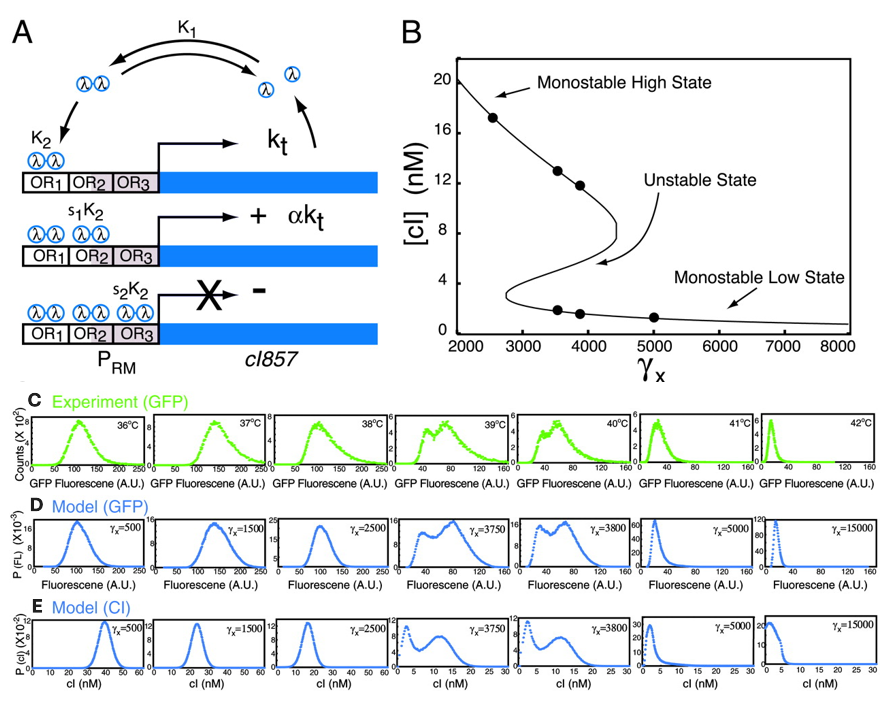
\includegraphics[width = 0.6\textwidth]{figura_mod.png}
\caption{Figura adaptada de \cite{Isaacs2003}. (A) La región promotora contiene tres sitios operadores (OR1-OR3). El gen cI857 expresa un represor ($\lambda$) que forma dímeros y se une a OR1 (expresión basal), OR2 (activación) y OR3 (represión). (B) Diagrama de bifurcación del modelo estocástico establecido. Se observa biestabilidad en rangos concretos de la tasa de degradación ($\gamma_x$). También se puede observar la bifurcación tipo silla-nodo. (C) Histogramas de fluorescencia (GFP, verde; unidades arbitrarias, A.U.) de cultivos con la red autoreguladora, normalizados por tamaño celular (experimental). (D-E) Simulaciones de GFP (azul, D) y represor cI (E) frente a variaciones de temperatura.}
\end{figure}

%%Contexto:
La mayoría de las funciones celulares resultan de la interacción entre genes, proteínas, RNAs y metabolitos a través de redes de regulación. Uno de los grandes desafíos de la biología de sistemas es ser capaz de deducir respuestas fenotípicas celulares a partir de la estructura y comportamiento de estas redes de interacción molecular tan complejas. Para ello, estas redes pueden diseccionarse en módulos más pequeños, unidades funcionales más sencillas (\cite{Hartwell1999}), cuya caracterización aislada facilita la predicción de comportamientos en redes complejas (\cite{Arnone1997}). El trabajo de Isaacs et al. ejemplifica este enfoque que se conoce como “bottom up”.
%¿Qué se sabía antes sobre la predicción de la expresión génica a partir de la secuencia?
%¿Qué limitaciones existían en los métodos anteriores?
%¿Por qué es relevante volver a examinar esta relación?

%%Contribución del estudio: 
Este estudio demuestra cómo un enfoque integrado en el que se combina un modelo cuantitativo junto con los componentes esenciales de una red, concretamente el módulo estudiado de regulación de los genes cI y cro del fago $\lambda$, permite descubrir propiedades clave de los sistemas biológicos como la biestabilidad o la presencia de histéresis. Esta combinación del enfoque teórico y experimental es clave para entender el funcionamiento de las redes reguladoras a gran escala como los patrones globales de expresión o la letalidad génica (\cite{Hartwell1999}).

Isaacs et al. demostraron que la desestabilización de la proteína mutante del represor $\lambda$ debida a la temperatura desencadenaba un régimen biestable dentro de una población celular que se mantenía gracias a la retroalimentación positiva del represor (cI). Esta biestabilidad sólo pudo modelarse mediante un modelo estocástico que era capaz de reflejar lo que sucede a nivel celular: el ruido génico se debe a fluctuaciones en el número absoluto de moléculas debido a la aleatoriedad de las reacciones químicas (\cite{Ozbudak2002}). Este trabajo refuerza la idea de que el ruido intrínseco, lejos de ser un artefacto, es un componente funcional en sistemas biológicos, capaz de impulsar transiciones entre estados estables sin necesidad de fluctuaciones externas. Esto conecta con trabajos de \cite{Elowitz2000} sobre ruido intrínseco/extrínseco en expresión génica, y subraya la función dual del ruido: a menudo considerado perturbador, aquí es un motor de cambio de estado programado.

%Uso de circuitos genéticos sintéticos con promotores diseñados racionalmente.
%Desarrollo de un modelo cuantitativo que relaciona secuencia y expresión.
%Prueba experimental en E. coli usando GFP como reportero.

%%Aspectos técnicos y metodológicos:
%Medición sistemática de niveles de fluorescencia para construir el modelo.
%Ajuste del modelo con regresión lineal y evaluación de su predictibilidad.
%Validación cruzada con nuevos promotores.

El módulo genético utilizado en este estudio está bien caracterizado (procedente del sistema regulador del fago $\lambda$), lo que facilitó la integración de parámetros bioquímicos ya establecidos (afinidad de unión del represor a los operadores y las tasas de dimerización proteica) en los modelos matemáticos desarrollados, dotando al modelo de un buen nivel de precisión biológica. La incorporación de fluctuaciones estocásticas mediante las ecuaciones de Langevin, que incorporan ruido interno debido al escaso número de moléculas en el sistema, permitió adaptar correctamente la distribución bimodal de los estados celulares observada experimentalmente. A diferencia de los enfoques que ajustaban de manera empírica un parámetro de ruido, el hecho de que ese modelo mecanicista haya podido replicar los histogramas de fluorescencia, las medias y los coeficientes de variación sin que hiciera falta calibraciones arbitrarias, pone de manifiesto la importancia de que los modelos que se utilicen para tratar de predecir comportamientos emergentes dentro de la biología sintética tengan que estar basados en mecanismos bioquímicos reales.

Este trabajo permitió establecer un precedente a nivel metodológico. Esto es porque combinaron herramientas complementarias: simulaciones estocásticas discretas (como el algoritmo de Gillespie, permitiendo modelar eventos moleculares individuales) con el análisis determinista continuo. Esta forma de integrar multiescala es importante para abordar sistemas donde coexisten procesos rápidos y lentos. Experimentalmente se realizaron mediciones sistemáticas de fluorescencia de GFP mediante el uso de citometría de flujo, cuantificando la expresión génica a nivel de células individuales. Los datos se ajustaron posteriormente al modelo utilizando regresión lineal, validando su capacidad predictiva al demostrar una correlación significativa entre las simulaciones y los resultados experimentales. Este enfoque que integra teoría, modelado estocástico y validación experimental refleja el potencial de los modelos basados en mecanismos para resolver la dinámica de las redes genéticas complejas.

%%Resultados relevantes:
%Se puede predecir la expresión con alta precisión en un rango amplio.
%Confirmación de que elementos de secuencia contribuyen de manera aditiva a la fuerza del promotor.
%Identificación de los sitios más determinantes para la actividad del promotor.

A su vez, demostró que es posible predecir y medir cuantitativamente la dinámica de un módulo genético autorregulador, concretamente una red de retroalimentación positiva. Mediante modelos teóricos (enfoque determinista y estocástico) y simulaciones se ha podido confirmar que los elementos de secuencia contribuyen de manera aditiva a la fuerza del promotor, identificando los sitios más determinantes para la actividad del promotor (arquitectura de retralimentación positiva).

%%Implicaciones:
%Permite diseño predictivo de promotores con fuerza deseada.
%Facilita el control preciso de la expresión génica en organismos modificados.
%Contribuye al paradigma de diseño de sistemas biológicos con lógica ingenieril.

%%Limitaciones:
%Hecho en un sistema simplificado (E. coli), sin considerar la complejidad de la regulación eucariota.
%No se incluyen efectos epigenéticos ni estructuras secundarias del ARN mensajero.
%El modelo es lineal y puede no captar todas las interacciones biológicas.

%Entre las limitaciones y desafíos que plantea el estudio se encuentran:
%\begin{itemize}
%    \item Escalabilidad: Mientras que módulos aislados son manejables, su acoplamiento en redes multicapa (ej., interacciones metabolismo-transcripción) introduce no linealidades impredecibles.
%    \item Contexto celular: El estudio usó plásmidos de alto número de copias, pero en sistemas genómicos nativos (copias únicas), el ruido y la dinámica podrían variar significativamente.
%    \item Estudio microscópico complementario: podría posibilitar la medición temporal transiciones en escalas de tiempo inferiores al tiempo de división de la célula, permitiendo la comparación directa del modelo experimental respecto al nivel unicelular, mientras que la tecnología utilizada en el estudio (citometría de flujo) proporciona únicamente estadísticas unicelulares en una población de células.
%    \item Aplicaciones \textit{in vivo}: La dependencia de la temperatura como interruptor limita su uso en organismos homeotérmicos. Alternativas (moléculas pequeñas, luz) requieren exploración.
%\end{itemize}

%Intento fusión:
Sin embargo, el estudio presenta varias limitaciones. Se empleó plásmidos de alto número de copias lo que no es representativo del fago $\lambda$ que sólo presenta una copia, por lo que el ruido y la dinámica podría variar significativamente de la realidad. Además, sólo se está caracterizando un módulo aislado de manera que al acoplarlo a redes multicapa podrían introducirse no linealidades que dieran lugar a un comportamiento impredecible por el modelo. Por otro lado, la citometría de flujo sólo proporciona estadísticas unicelulares a través de una población de células. De esta manera, haber desarrollado un estudio microscópico celular que permitiera la medición a tiempo real de las transiciones que ocurren en escalas de tiempo inferiores al tiempo de división celular habría permitido la comparación directa entre el modelo y el experimento a nivel unicelular. En el caso de querer emplear este módulo en organismos eucariotas, se debería considerar la complejidad de la regulación eucariota desde efectos epigenéticos a las estructuras secundarias del ARN mensajero. Además, su uso estaría limitado en organismos homeotermos sensibles al cambio de temperatura.

%%Proyecciones futuras:
%Aplicaciones en diseño de terapias génicas o biosensores.
%Extensión a otros organismos y redes génicas más complejas.
%Integración con aprendizaje automático y modelos más sofisticados.

Este trabajo dio lugar un gran número de estudios sobre la dinámica estocástica en la biología, inspirando formas de modelar, medir y diseñar sistemas genéticos. Hoy la ingeniería de circuitos sintéticos incluye el ruido como un parámetro más del diseño y se reconoce el papel fundamental que el ruido desempeña en el desarrollo, en la diferenciación o en la resistencia a tratamientos. Este artículo también anticipó una visión más rica y más realista de la biología molecular, donde el determinismo se mezclaba con la probabilidad para dar lugar a un comportamiento complejo, diverso y evolutivamente robusto.

%%Reflexión/Crítica:
%¿Qué aporta este enfoque a la biología computacional moderna?
%¿Qué impacto ha tenido desde su publicación (2003)?
%¿Qué desafíos siguen abiertos respecto a la predicción de expresión génica?

En conclusión, el trabajo de Isaacs et al. se considera un avance en el terreno de la caracterización cuantitativa de módulos genéticos. Al emplear modelos estocásticos junto con valores conocidos permite no sólo validar principios teóricos, sino también proporcionar un marco para el diseño de circuitos sintéticos con funciones predecibles. La perspectiva futura pasa por la caracterización de las dinámicas de la conmutación a nivel unicelular, la evaluación de los efectos de contexto o la búsqueda de acoplamientos modulares, acercándonos así al objetivo de diseñar redes de regulación génica con capacidades de predicción precisas.

\printbibliography

\end{document}